\chapter{Vacuum Energy, Unification, and Grassmann Superspace}

These notes follow Leonard Susskind's sixth lecture in the supplementary course on supersymmetry and grand unification, with curation by LazyingArt LLC. The lecture does not begin by plunging deeper into superspace. Instead, it comes back to supersymmetry through a student question about the Casimir effect, uses that question to sharpen what we mean by vacuum energy, then turns to what supersymmetry actually does, why low-energy supersymmetry might matter, why cosmology forces us to think more carefully about energy, and finally what sort of Grassmann calculus is needed if supersymmetric theories are to be written in a compact and reliable way.

\section{Vacuum Energy, Casimir Effect, and Honest Evidence}

We enter through the Casimir effect because that is how the lecture itself reenters the subject. Take two reflecting plates a distance \(L\) apart. In empty space there are vacuum fluctuations, or if one prefers, zero-point oscillators associated with the quantum fields. Once the plates are inserted, those vacuum processes are modified. Virtual loops that would have occupied the region freely are interrupted by the reflecting boundaries, and the vacuum energy becomes a function of the plate separation.

That is already enough to produce a force. If the energy depends on \(L\), we may read it as a potential energy, and then the force is obtained by differentiation:
\begin{equation}
F(L)=-\frac{dE_{\mathrm{Casimir}}(L)}{dL}.
\end{equation}
This is the point Susskind wants first: the Casimir effect is a quantum-field-theoretic force coming from the dependence of vacuum energy on boundary conditions. The lecture does not stabilize the exact power law in \(L\), and we should not pretend otherwise. What matters here is the logic, not the detailed coefficient.

For the electromagnetic vacuum the force is typically attractive. Susskind adds, cautiously, that if the relevant loop were fermionic the sign would go the other way. The important lesson is that the sign can depend on the field content, while the mechanism itself is general: the plates alter the vacuum modes, and altered vacuum modes mean altered energy.

But then he immediately refuses to let the Casimir effect do more conceptual work than it deserves. Yes, it is often advertised as evidence for vacuum energy, but it is also possible to think of it more modestly as a force between nearby plates. If we ask for \emph{honest} evidence that vacuum energy is really there as energy, then we must ask what energy does most fundamentally. It gravitates. The serious question is not whether vacuum loops shift a force in the laboratory, but whether the energy of empty space contributes to gravitation.

That is the pivot to cosmology. The energy of empty space does gravitate, and in the lecture the clean statement is that the real evidence for vacuum energy is the accelerated expansion of the universe. The Casimir effect is suggestive; cosmological acceleration is the honest gravitational evidence.

\subsection{Question \& Answer}

\paragraph{Question.} What is actually mysterious about vacuum energy?

\paragraph{Answer.} Not its existence. In the lecture Susskind is emphatic about this point. Quantum field theory predicts zero-point energy for every field. In that sense vacuum energy is not obscure at all; it is built into the formalism. What is mysterious is that the observed vacuum energy is so tiny. For many years physicists persuaded themselves that it must vanish exactly, because the observed value was so much smaller than naive field-theoretic estimates. The surprise of modern cosmology is not that vacuum energy exists, but that it is so suppressed and yet not zero.

That distinction matters for the whole chapter. We are not trying to explain why empty space has energy at all. We are trying to understand why the amount that gravitates is so feeble.

\section{What a Supersymmetry Generator Really Does}

The next student question forces a clarification that is easy to lose if one speaks too loosely about bosons turning into fermions. Suppose many bosons occupy the same state. If we apply a supersymmetry transformation, do we suddenly create a forbidden pile of fermions in one state? Susskind's answer is no, and the reason is built into the character of the generator.

He denotes the supersymmetry generator by \(Q\). It is a fermionic generator, not an ordinary rotation generator. A rotation generator can be compounded over and over again; repeated infinitesimal actions build a finite rotation. That is not how \(Q\) behaves. Its action is local in fermion number. It removes one boson and replaces it by one fermion, or removes one fermion and replaces it by one boson:
\begin{equation}
Q\,|B\rangle \propto |F\rangle,
\qquad
Q\,|F\rangle \propto |B\rangle,
\qquad
Q^2=0.
\end{equation}
The last relation is the crucial one for the lecture. Because \(Q\) is nilpotent, one cannot simply keep acting with it until a macroscopic bosonic population has been converted into a fermionic one. The second action gives zero. In the language Susskind uses, supersymmetry changes us by one unit of fermion number.

This is exactly the sort of local algebraic point that would be flattened away in a more textbook-like summary, but here it is pedagogically central. A conceptual obstacle is raised and then removed before the lecture goes on to motivation.

\subsection{Question \& Answer}

\paragraph{Question.} Why can repeated action of \(Q\) not turn a Bose population into a Fermi population?

\paragraph{Answer.} Because the supersymmetry generator is not an ordinary bosonic generator that can be compounded indefinitely. Its square vanishes:
\begin{equation}
Q^2=0.
\end{equation}
So the action of \(Q\) is not “replace every boson by a fermion.” It is “replace one by one,” and the algebra prevents the iteration from building up a large finite transformation of the kind we are used to from spatial rotations.

\section{Why Low-Energy Supersymmetry Is Worth Taking Seriously}

Only after this clarification does the lecture ask directly what supersymmetry may buy us phenomenologically. Susskind is careful to restrict the claim: by supersymmetry here he means supersymmetry low enough in scale to matter for experiments not too far beyond present reach. With that understood, he organizes the middle of the lecture around three motivations:
\begin{enumerate}
\item control of the Higgs self-energy;
\item stable new particles, especially dark-matter candidates;
\item higher-precision unification.
\end{enumerate}
The third motivation belongs naturally with running couplings, so we hold it for the next section. The first two are developed immediately.

\paragraph{The Higgs self-energy problem.}
The lecture phrases the problem qualitatively, in terms of large self-energy corrections. Vacuum fluctuations attached to the Higgs line shift the Higgs mass upward. If there were nothing to protect it, the Higgs mass would be dragged to a very high scale. Since the masses of the ordinary particles are responses to the Higgs phenomenon, they would be dragged upward as well. The whole low-energy world would be destabilized.

Susskind does not derive loop formulas here, and we should not insert them gratuitously. The point is structural. Bosonic and fermionic contributions come with opposite tendencies, and supersymmetry organizes the cancellations. If the symmetry is present at a low enough scale, the dangerous Higgs self-energy corrections are controlled.

\paragraph{Stable superpartners and dark matter.}
The second motivation is more physical than algebraic. If there are ordinary particles and superpartners, then a decay that begins with a superpartner always leaves a superpartner behind. Schematically,
\begin{equation}
\tilde X \rightarrow X+\tilde Y \rightarrow X+Y+\tilde Z \rightarrow \cdots
\end{equation}
and the chain cannot end in purely ordinary particles. Therefore there is a lightest superpartner, the LSP, and in the simple version of the story it is stable.

That is immediately suggestive for dark matter. Dark matter is believed to be particulate, long-lived on cosmological time scales, and only weakly coupled to ordinary matter. A stable superpartner is exactly the kind of object that could play that role. The lecture stresses that if dark matter were strongly coupled or electrically charged, it would scatter, lose energy, and collapse toward the visible matter distribution rather than remaining in the extended galactic halo. So the candidate must be weakly interacting, and likely neutral.

Susskind also preserves the cosmological intuition: in the early hot universe one expects thermal equilibrium to populate ordinary particles and superparticles comparably, until the heavier unstable states decay away. If the LSP is stable, some relic abundance can remain. He is careful not to overstate this. The lecture does not derive a relic-density formula; it gives the qualitative argument that supersymmetry naturally supplies the right sort of object.

\section{Running Couplings and Higher-Precision Unification}

The third motivation begins from renormalization rather than from symmetry. Electric charge is screened. At shorter distances, or equivalently higher energies, the effective electromagnetic coupling grows. Susskind prefers to plot the inverse coupling because in the simplest approximation it is nearly linear:
\begin{equation}
\alpha_{\mathrm{em}}^{-1}(E) \ \text{falls as } E \text{ increases}.
\end{equation}
The electroweak coupling behaves similarly, with a different slope. The strong coupling behaves in the opposite way because of asymptotic freedom:
\begin{equation}
\alpha_s^{-1}(E) \ \text{rises as } E \text{ increases}.
\end{equation}
The lecture's image of running is resolutely Feynman-diagrammatic. The charge seen at large distance is modified by loops. A photon exchanged between two charged particles can contain an electron-positron loop. When we come to short enough distances, there is, so to speak, no room for that loop, and the effective charge changes. Running is not an abstract bookkeeping device; it is the physical accumulation of loop effects.

This is exactly where supersymmetry reenters. Once superpartners are added to the theory, new loops appear, and the slopes of the running couplings change. In the unmodified Standard Model the three gauge couplings tend in the same direction, but they miss one another by too much to make a convincing single crossing. With superpartner loops included, the extrapolation improves strikingly:
\begin{equation}
\alpha_{\mathrm{em}}^{-1}(E_U)\approx
\alpha_{\mathrm{ew}}^{-1}(E_U)\approx
\alpha_s^{-1}(E_U),
\qquad
E_U\sim 10^{15}\text{--}10^{16}\,\mathrm{GeV}.
\end{equation}
No one has measured physics at that scale. The statement is an extrapolation using the measured low-energy couplings and the loop structure of the theory. But this is precisely why Susskind calls it higher-precision unification: two lines crossing is easy to arrange; three meeting cleanly at one point is much harder to dismiss as happenstance.

The lecture then adds the necessary qualification. This picture only works if the superpartners are not too heavy. If their masses are pushed far upward, their loops do not influence the running early enough, the three lines miss, the Higgs cancellation is weakened, and the dark-matter scale drifts away from the appealing TeV-ish regime. Thus the three motivations are not independent. They all lean toward low-energy supersymmetry in roughly the same range.

As an aside, Susskind also remarks that a gravitational coupling, defined heuristically, would strengthen with energy because gravitational charge is energy. Its inverse would therefore fall with energy and cross not too far away. He is cautious here, and so should we be. The lecture treats this as suggestive, not as a sharp unification theorem.

\section{Vacuum Energy in Cosmology and the Friedmann Balance}

At this point the lecture turns by way of another student question: what is the difference between the Higgs divergence and the vacuum-energy divergence? The answer is that vacuum-energy diagrams are just virtual processes in empty space. Higgs self-energy diagrams are vacuum processes modified by the presence of the Higgs particle itself. The Higgs is treated, in one of Susskind's nicest phrases, as an impurity in the vacuum. The impurity changes the vacuum fluctuations attached to its line, and that shifted cloud alters the particle's mass.

This distinction leads straight into cosmology, because vacuum energy has one special feature that ordinary matter and radiation do not share. As the universe expands, the energy density in non-relativistic matter falls because the number of particles in a comoving region stays fixed while the volume grows. Radiation falls even faster, because the expansion stretches wavelengths and lowers the energy of each quantum. Vacuum energy does not dilute.

The lecture states this verbally. The clean mathematical version is
\begin{equation}
\rho_{\mathrm{matter}}\propto a^{-3},
\qquad
\rho_{\mathrm{radiation}}\propto a^{-4},
\qquad
\rho_{\mathrm{vacuum}}=\text{constant}.
\end{equation}
Here \(a(t)\) is the cosmological scale factor, which Susskind treats informally as the radius or expansion factor of the universe.

\begin{figure}[t]
\centering

\includegraphics[width=0.58\textwidth]{lecture_06_figure_03.png}
\caption{Geometry equals energy in the cosmological equation.}
\end{figure}

This is the point at which the blackboard slogan appears: geometry equals energy. The first visible term is the expansion term \(\left(\dot a/a\right)^2\), and the lecture now rewrites the cosmological dynamics as a balance between geometry on the left and energy content on the right.

A cautious cleaned-up version of the board structure is
\begin{equation}
\left(\frac{\dot a}{a}\right)^2 \pm \frac{1}{a^2}
\longleftrightarrow
\rho_{\mathrm{matter}}+\rho_{\mathrm{radiation}}+\rho_{\mathrm{vacuum}},
\qquad
\rho_{\mathrm{matter}}=\rho_{\mathrm{ordinary}}+\rho_{\mathrm{dark}}.
\end{equation}

\begin{remark}
The lecture and the selected frames fix the structure of this equation more securely than its normalization. We therefore keep the board-level form visible and do not import coefficients that were not established in the lecture. The sign of the curvature term depends on whether the universe is open, closed, or flat.
\end{remark}

\begin{figure}[t]
\centering

\includegraphics[width=0.88\textwidth]{lecture_06_figure_04.png}
\caption{Friedmann balance of expansion, curvature, and energy content.}
\end{figure}

\begin{figure}[t]
\centering
\begin{tikzpicture}
\draw (-1.6,1.4) rectangle (1.6,-0.2);
\draw (3.0,1.6) rectangle (8.2,-0.4);
\node at (0,1.0) {$\left(\frac{\dot a}{a}\right)^2$};
\node at (0,0.2) {$\pm\,\dfrac{1}{a^2}$};
\node at (0,-0.8) {geometry};
\node at (2.3,0.6) {$=$};
\node at (5.6,1.0) {$\rho_{\mathrm{matter}}+\rho_{\mathrm{radiation}}+\rho_{\mathrm{vacuum}}$};
\node at (5.6,0.2) {$\rho_{\mathrm{matter}}=\rho_{\mathrm{ordinary}}+\rho_{\mathrm{dark}}$};
\node at (5.6,-1.0) {energy};
\end{tikzpicture}
\caption{Schematic reconstruction of the board balance: geometry on the left, cosmic contents on the right.}
\end{figure}

This detour is not decorative. It sharpens the meaning of vacuum energy. Because \(\rho_{\mathrm{vacuum}}\) does not dilute, a component that was negligible in the early universe eventually dominates. That is the lecture's explanation for why vacuum energy is now cosmologically important even though it was subdominant in the past. In the lecture's approximate language, the present cosmic budget is about \(70\%\) vacuum energy and \(30\%\) everything else.

\subsection{Question \& Answer}

\paragraph{Question.} How can energy be conserved if vacuum energy density does not dilute as the universe expands?

\paragraph{Answer.} The lecture's answer is deliberately startling: in this cosmological setting the total energy is constrained to be exactly zero. One should not read this as a blanket statement about every spacetime. It is a statement about the cosmological Einstein equation being used here.

Susskind phrases the time-time Einstein equation as a balance between geometry and energy. If we move everything to one side, the result is read as a Hamiltonian constraint:
\begin{equation}
H_{\mathrm{tot}}=0.
\end{equation}
Schematically, one may write
\begin{equation}
\left(\frac{\dot a}{a}\right)^2 \pm \frac{1}{a^2}
-
\left(
\rho_{\mathrm{matter}}+\rho_{\mathrm{radiation}}+\rho_{\mathrm{vacuum}}
\right)
=0.
\end{equation}
In the lecture this is interpreted as saying that the ordinary positive forms of energy are compensated by geometric terms associated with expansion and curvature. If one insists on speaking in ordinary energy language, the compensating geometric contribution behaves like a negative expansion energy. The important point is not a Newtonian picture of bookkeeping, but the general-relativistic constraint: once the whole cosmological system is written correctly, the canonical Hamiltonian vanishes.

\section{Grassmann Numbers, Superspace, and Superfields}

Only after the cosmology tangent has run its course does the lecture return explicitly to supersymmetry. A student asks whether Grassmann numbers appear in the Lagrangian. Susskind's answer is yes, in two distinct ways.

First, fermion fields themselves are Grassmann-valued. Bosonic fields are ordinary-number-valued; fermionic fields anticommute. That fact is already familiar from field theory. The second appearance is deeper and more characteristic of supersymmetry: one introduces extra coordinates \(\theta\), Grassmann coordinates, so that supersymmetric theories can be organized in an enlarged space built from ordinary coordinates and anticommuting ones.

The lecture describes this almost geometrically. Besides the ordinary coordinates \(x^\mu\), we introduce two complex, or equivalently four real, Grassmann coordinates. They are not large extra dimensions in the ordinary sense. They are nilpotent:
\begin{equation}
\theta^2=0.
\end{equation}
That is why Susskind says they are small. One cannot roam around them as one roams through ordinary space. But they are enough to organize bosons and fermions into a single bookkeeping object, the superfield.

Ordinary fields are functions of \(x\). Superfields are functions of \(x\) and \(\theta\):
\begin{equation}
\Phi=\Phi(x,\theta).
\end{equation}
Because the \(\theta\)'s are nilpotent, the expansion in Grassmann variables terminates after finitely many terms. In the four-real-theta version used for orientation in the lecture, a schematic expansion is
\begin{equation}
\Phi(x,\theta)
=
\phi(x)
+\theta_\alpha\psi_\alpha(x)
+\theta_\alpha\theta_\beta z_{\alpha\beta}(x)
+\cdots
+\theta_1\theta_2\theta_3\theta_4\,D(x).
\end{equation}
This is not yet a convention-heavy superspace formalism. It is a clean bookkeeping statement. A superfield is a finite multiplet of ordinary component fields, alternating in bosonic and fermionic character according to the number of \(\theta\)'s carried by each term.

Once this is accepted, the next structural step is immediate. A supersymmetric Lagrangian density is also a function of \(x\) and \(\theta\), built from superfields and their derivatives, and the action must be obtained by integrating over both:
\begin{equation}
S=\int d^4x\,d^4\theta\,\mathcal{L}(x,\theta).
\end{equation}
That raises the next question in exactly the right way. Ordinary integration over spacetime is familiar. What can it possibly mean to integrate over Grassmann variables?

\section{Grassmann Integration as the Calculus of Supersymmetry}

The lecture answers this by first recalling a very ordinary fact and then imitating it in a strange setting.

\begin{figure}[t]
\centering

\includegraphics[width=0.86\textwidth]{lecture_06_figure_05.png}
\caption{Definite integral of a derivative.}
\end{figure}

For ordinary functions we use the definite integral of a total derivative:
\begin{equation}
\int_{-\infty}^{\infty}\frac{dF}{dx}\,dx
=
F(\infty)-F(-\infty)
=
0,
\end{equation}
provided the function dies off at large positive and negative \(x\). This is the board identity Susskind writes before turning to Grassmann variables. It is not a random review. It is the model for what the Grassmann integral is supposed to preserve: the definite integral of a derivative should vanish.

\subsection{Question \& Answer}

\paragraph{Question.} What do we mean by integrating over Grassmann variables?

\paragraph{Answer.} We do \emph{not} mean an indefinite integral, and we do not mean a sum of infinitesimal areas. In the lecture the Grassmann integral is defined as a definite integral over the whole theta-space, fixed by a small number of useful rules. Its content is algebraic, not geometric in the usual sense.

For one Grassmann variable \(\theta\), Susskind's construction runs as follows:
\begin{enumerate}
\item Demand linearity of the integral.
\item Impose the analog of the ordinary total-derivative rule,
\[
\int d\theta\,\frac{d}{d\theta}f(\theta)=0.
\]
\item Take \(f(\theta)=\theta\). Since \(\dfrac{d}{d\theta}\theta=1\), this gives
\begin{equation}
\int d\theta\,1=0.
\end{equation}
\item Fix the remaining normalization by convention:
\begin{equation}
\int d\theta\,\theta=1.
\end{equation}
\end{enumerate}
That is already the whole table for one Grassmann variable, because every function of one \(\theta\) has the form
\begin{equation}
f(\theta)=a+b\theta.
\end{equation}
Hence
\begin{equation}
\int d\theta\,f(\theta)=\int d\theta\,(a+b\theta)=b.
\end{equation}
So the Grassmann integral simply picks out the coefficient of the highest theta term. In this one-variable case it is even identical to the derivative:
\begin{equation}
\int d\theta\,(a+b\theta)=b=\frac{d}{d\theta}(a+b\theta).
\end{equation}

This also explains why there is no indefinite integral in the ordinary sense. There is no function whose derivative is \(\theta\), because that function would have to contain \(\theta^2\), and \(\theta^2=0\). The lecture uses this as part of the warning that one should not try to divide by \(\theta\).

For two Grassmann variables, which Susskind writes as \(\theta\) and \(\bar\theta\), the general function is
\begin{equation}
f(\theta,\bar\theta)=a+\bar\theta\psi+\bar\psi\,\theta+b\,\bar\theta\theta.
\end{equation}
There are only four terms because \(\theta^2=\bar\theta^2=0\). If we choose the measure ordering
\begin{equation}
\int d\theta\,d\bar\theta\,\bar\theta\theta=1,
\end{equation}
then every term except the top component integrates to zero, and therefore
\begin{equation}
\int d\theta\,d\bar\theta\,f(\theta,\bar\theta)=b.
\end{equation}

\begin{remark}
Ordering matters. The lecture visibly struggles with the sign at the board and corrects it in real time. With the convention adopted here,
\[
\int d\bar\theta\,d\theta\,\bar\theta\theta=-1.
\]
Reversing the order of either the variables or the measure changes the sign.
\end{remark}

This is the whole conceptual payoff. Integrating over the \(\theta\)'s means extracting the highest Grassmann component. What sounds almost trivial is powerful because it provides a calculus for writing interacting supersymmetric Lagrangians while preserving the delicate boson-fermion cancellations that motivated the subject in the first place. That is the point of the construction. It is not an ornamental formalism; it is the bookkeeping machinery that keeps supersymmetry intact when the theory becomes complicated.

\section{Summary}

The lecture begins with the Casimir effect, but only to ask what would count as real evidence for vacuum energy. From there it clarifies that the mystery of vacuum energy lies in its tiny size, not in its existence, then turns to what the supersymmetry generator really does, why low-energy supersymmetry is attractive for Higgs naturalness, dark matter, and unification, why cosmology forces us to reinterpret energy through a Friedmann balance and a Hamiltonian constraint, and finally how superspace and Grassmann integration provide the calculus needed to build supersymmetric theories. The chapter has therefore ended where the lecture ends: not with a finished model, but with the formal machinery now laid out so that explicit constructions can begin.